%%%%%%%%%%%%%%%%%%%%%%%%%%%%%%%%%%%%%%%%%
% Medium Length Professional CV
% LaTeX Template
% Version 2.0 (8/5/13)
%
% This template has been downloaded from:
% http://www.LaTeXTemplates.com
%
% Original author:
% Trey Hunner (http://www.treyhunner.com/)
%
% Important note:
% This template requires the resume.cls file to be in the same directory as the
% .tex file. The resume.cls file provides the resume style used for structuring the
% document.
%
%%%%%%%%%%%%%%%%%%%%%%%%%%%%%%%%%%%%%%%%%

%----------------------------------------------------------------------------------------
%	PACKAGES AND OTHER DOCUMENT CONFIGURATIONS
%----------------------------------------------------------------------------------------

\documentclass{resume} % Use the custom resume.cls style

\usepackage[left=0.75in,top=0.5in,right=0.75in,bottom=0.5in]{geometry} % Document margins
\usepackage{hyperref}
\usepackage{array} 
\usepackage{textpos}
\usepackage[utf8]{inputenc}
\usepackage{graphicx}
\usepackage{enumitem}
\usepackage[russian,english]{babel}
\setcounter{secnumdepth}{4}

\begin{textblock}{7}(0, 0.05)
    {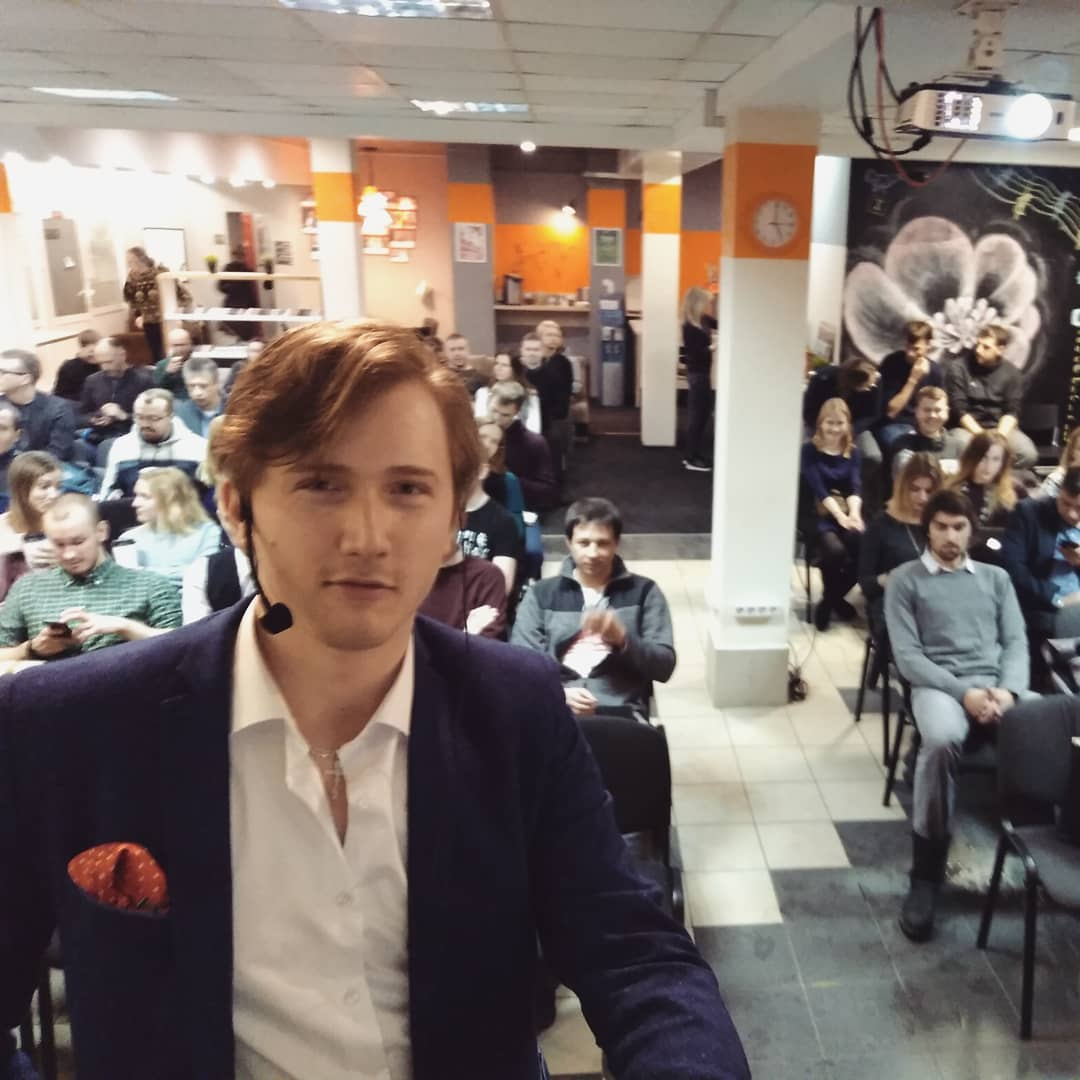
\includegraphics[width=.25\linewidth]{photo.jpg}}
\end{textblock}

\name{Alexander Mikhalchenko} % Your name
\address{Belarus, Minsk 220113} % Your address
\address{Linkedin: \href{http://linkedin.com/in/mikhalchenkoa}{linkedin.com/in/mikhalchenkoa} \\ StackOverflow: \href{http://stackoverflow.com/users/2044039}{id 2044039}} \\
\address{strrife@gmail.com \\ skype:strrife } % Your phone number and email

\begin{document}

%----------------------------------------------------------------------------------------
%	SUMMARY SECTION
%----------------------------------------------------------------------------------------

\begin{rSection}{Summary}

Over the past years I have worked in multiple international companies and proven
myself to be the guy that can save the project. If you're looking for someone who'd be able to rock it starting from DB
architecture (MySQL, MongoDB, Redis, Elasticsearch) to backend (NodeJS, PHP, Java) and, of course, frontend
(Javascript, ES5, ES6, Angular, Aurelia), you're reading the right CV.

I have a strong mathematical background (see Honors & Awards section) and I prefer to work in R\&D where I can show my best.
Also, during the past year I've been slowly moving towards management and IT sales. I'm an empathic communicator, good at pitching.

\end{rSection}


%----------------------------------------------------------------------------------------
%	TECHNICAL STRENGTHS SECTION
%----------------------------------------------------------------------------------------

\begin{rSection}{Technical Strengths}

\begin{tabular}{ @{} >{\bfseries}l @{\hspace{4ex}} l }
JavaScript  & ES6, Angular, Aurelia, jQuery, JSPM, Bower, Babel \\
NodeJS  & NPM, Express, Grunt, Gulp, Yeoman, Isomorphic apps, Browserify \\
PHP & PHP7, Symfony (1.4, 2.5), Wordpress, Silex, Composer, Doctrine, PDO \\
Databases & MySQL, MongoDB, ElasticSearch, MapReduce, Redis, SQLite, SQLPlus \\
HTML/CSS & HTML5, Canvas, SASS/LESS, CSS3, Bootstrap, Flat UI \\
Testing & Unit tests, Integration tests, Mocha, Karma, Selenium, Nightmare.js \\
Other & AWS, Python, Groovy
%VCS & Git, Perforce \\
\end{tabular}

\end{rSection}

%----------------------------------------------------------------------------------------
%	WORK EXPERIENCE SECTION
%----------------------------------------------------------------------------------------

\begin{rSection}{Experience}


\begin{rSubsection}{TractionBoard}{March 2016 - Present}{CTO}{}
\item Working on Aurelia-based frontend and Symfony-based backend
\item BigData processing (ElasticSearch Scripting - Groovy) and visualization (D3)

\begin{rSubsection}{Severex}{November 2015 - Present}{Senior Frontend Developer (Aurelia)}{}
\item Working on Aurelia-based frontend, BigData visualization
\end{rSubsection}

%------------------------------------------------

\begin{rSubsection}{DualLab}{August 2015 - December 2015}{Full-stack Web Developer}{}
\item Single-handedly developed the backend (Node.js, TDD)
\item Actively participated in frontent development (Angular)
\item For recommendations from teamlead \& colleagues see my \href{http://linkedin.com/in/mikhalchenkoa}{linkedin profile}

%{\bf Projects}:
%
%\begin{itemize}[leftmargin=*,label={$+$}]
%  \item {\bf REST API}.  Created API on top of the existing legacy gSOAP API
%  \item {\bf Web client}. Worked on the prototype for the web client.
%\end{itemize}

\end{rSubsection}

%------------------------------------------------

\begin{rSubsection}{StarOfService}{April 2014 - August 2015}{Full-stack Web Developer}{}
\item Worked both on backend (PHP, Symfony 1.4) and frontend (Angular)
\item AWS integration (SQS, S3 integration)
\item RESTFul API development
\item Single-handedly developed and maintained primary search engine (TF-IDF based)
\item For recommendations from CEO, CTO \& teamlead see my \href{http://linkedin.com/in/mikhalchenkoa}{linkedin profile}

%{\bf Projects}:
%
%\begin{itemize}[leftmargin=*,label={$+$}]
%  \item {\bf AWS integration} (SQS, S3 integration)
%  \item {\bf Sherlock} (TF-IDF search engine for service lookup)
%  \item {\bf API} for the \href{https://itunes.apple.com/fr/app/starofservice/id948344674?mt=8}{iPhone app}
%  \item {\bf Request moderation tool} (user scoring system, request similarity algorithms)
%  \item {\bf Data mining and analysis tools} (Mixpanel, funnel setup, stats monitor: d3, Highcharts)
%  \item {\bf UI} (Implemented new signup, search for pros \& requests: Angular, Bootstrap).
%\end{itemize}

\end{rSubsection}

%------------------------------------------------

\begin{rSubsection}{Athena Art}{February 2014 - January 2016}{Wordpress Developer, Consultant}{}
%Actually I just don't want "thelordofporn" be in my cv. I though about it alot and decided that I'd rather ommit the name.  %
\item Did lots of Worpress customization
\item Site speed and Caching enchantments (from 1.5s to 30ms for homepage)
%
%%{\bf Projects}:
%
%\begin{itemize}[leftmargin=*,label={$+$}]
%  \item {\bf Wordpress Custom post type manager}
%  \item {\bf Speed optimization} (Custom Redis-based caching solution)
%\end{itemize}

\end{rSubsection}
\clearpage

%------------------------------------------------

\begin{rSubsection}{Itransition}{October 2013 - January 2014}{Fullstack Web developer intern (PHP, C\#)}{}
\end{rSubsection}

%------------------------------------------------

\begin{rSubsection}{Personal projects}{}{}

\begin{itemize}[leftmargin=*,label={$+$}]
  \item {\bf \href{http://nagibator.xyz}{VOUFF (ex Nagibator)}} \hfill {\em November 2015 - March 2016}  \\
	Live image tracking and replacement in videos. 2nd prize at Garage
	48 hackaton (Nov 2015), participated in TechMinsk Accelerator (Feb 2016).

  \item {\bf \href{http://gendalf.tv}{Gendalf TV}} \hfill {\em December 2015 - April 2016}  \\
	App for sending videos to LG Smart TV, 1st place at LG Hackaton (Dec 2015).
%
%  \item {\bf \href{http://toto.by}{ToTo.by}} \hfill {\em November 2015}  \\
%	Car-related information aggregator for Belarus.
%
%  \item {\bf \href{http://boxinator.xyz}{Boxinator}} \hfill {\em September 2015} \\
%	Cloud-based workflow management system, participant of Minsk FinTech hackaton.
%
%  \item {\bf \href{http://mmopricefinder.com}{MMOPriceFinder.com}} \hfill {\em July 2014} \\
%	WoW, FIFA and other games inner currency rates search.

\end{itemize}
\end{rSubsection}
\end{rSection}
%----------------------------------------------------------------------------------------

%----------------------------------------------------------------------------------------
%	EDUCATION SECTION
%----------------------------------------------------------------------------------------

\begin{rSection}{Education}
{\bf Belarussian State University, Belarus} \hfill {\em 2012 $-$ Present} \\
Bachelor Degree in Computer Science, minor in Intelligent Control Systems \hfill {\em Average: 9.4} \\
Courses taken: Algorithms, Pattern recognition, Natural Text Processing, Calculus, etc.

{\bf Belarussian State University Lyceum, Belarus} \hfill {\em 2010 $-$ 2012} \\
Associate degree in Mathematics \hfill {\em Average: 9.8}

\end{rSection}

%----------------------------------------------------------------------------------------
%	Mathematics
%----------------------------------------------------------------------------------------

\begin{rSection}{Honors \& Awards section}

\begin{rSubsection}{International Tournaments of Young Mathematicians}{}{}

\item ITYM 4 $-$ 1st place \& gold medal \hfill July 2012, Paris, France
\item ITYM 6 $-$ 2nd place \& gold medal (team leader) \hfill July 2014, Bremen, Germany

\end{rSubsection}

\begin{rSubsection}{Belarussian Mathematical Olympiads}{}{}

\item 61st BMO $-$ I diploma \hfill  April 2011, Belarus, Gomel
\item 62nd BMO $-$ II diploma \hfill April 2012, Belarus, Gomel
\end{rSubsection}


\begin{rSubsection}{Local Tournaments of Young Mathematicians}{}{}

\item XIV Belarussian TYM $-$ 1st place (team leader) \hfill December 2012, Belarus, Minsk
\item XV Belarussian TYM $-$ 1st place (team leader) \hfill December 2013, Belarus, Minsk
\item 2nd St.Petersburg TYM $-$ 1st place (team leader) \hfill March 2014, Russia, St. Petersburg
\end{rSubsection}

\end{rSection}

\begin{rSection}{Public Speaking & Publications}

    \begin{rSubsection}{Presentations at local meetups}{}{}

    \item Interracting with websites w/o API \hfill WebNotBombs conf, Minsk, Feb 2016
    \item Aurelia vs Angular 2 \hfill The Rolling Scopes \#21, Minsk, Dec 2015

    \end{rSubsection}

    \begin{rSubsection}{Publications}{}{}

    \item Sentimental corpus \& Semantic Web problems in tourism domain \hfill 72nd BSU Scientific Conference
    \item Plant Phenomics and Image processing Algorithms \hfill 73rd BSU Scientific Conference
    % ("Система синтеза сентиментального корпуса текста для решения задач semantic web в области туризма")%.
    \item Decision support systems and plant phenomics \hfill PRIP'16
    \item \href{http://textlab.io/doc/8452214}{Designing the platform for phenotyping stem cuttings and clones of ornamental woody plants}
    \end{rSubsection}
\end{rSection}


%----------------------------------------------------------------------------------------
%	EXAMPLE SECTION
%----------------------------------------------------------------------------------------

%\begin{rSection}{Section Name}

%Section content\ldots

%\end{rSection}

%----------------------------------------------------------------------------------------

\end{document}
